\subsection{$ G$の実階数が1の場合}

\begin{thm}\label{thm:1216-main}
  $G$を実階数1の実半単純Lie 群とするとき,\Cref{yosou:1121}が成り立つ.
\end{thm}

\begin{thm}\label{thm:0810}\cite[p.~409, Theorem~3.1]{hel01}

  $\ge = \ka \oplus \pe$を実半単純Lie環とそのCartan対合$\theta$に対する Cartan分解とし,$\alpha,2\alpha\in \Sigma(\ge,\ah) $と仮定する.このとき,$X_{\alpha},X_{2\alpha}, \theta X_{\alpha}, \theta X_{2\alpha} $から生成されるLie環$\ge^{*} $は$\sulie(2,1)$と同型である.
  
\end{thm}
以下で\Cref{thm:0810}を示すための補題や記号を設定し,\Cref{thm:0810}を示す.
\begin{nttdef}
  \leavevmode
  \vspace{-1em}
  \begin{itemize}
  \item $\ah \subset \ge$を極大分裂可換代数,$\emm \defeq \zet_{\ka}(\ah) \defeq \{W\in \ka\mid [W,\ah] = \{0\} \} $とする.$B$を$\ge$のKilling 形式とする.
  \item $\Sigma(\ge,\ah) $を$\ah$に関する制限ルート系とする.$\ge_{\lambda} $を,$\lambda\in \ah^{*}$のルート空間とし,$0\neq X_{\alpha}\in \ge_{\alpha} $,$0\neq X_{2\alpha}\in \ge_{2\alpha} $を任意に固定する.$Y_{\alpha}\defeq [\theta X_{\alpha}, X_{2\alpha}] $とする.
  \item $A_{\alpha}\in \ah $を,任意の$H\in \ah$に対して$B(H,A_{\alpha}) = \alpha(H) $を満たす元とする.
    
    このとき,任意の$H\in \ah$に対して$B(H, [X_{\alpha}, \theta X_{\alpha}]) = \alpha(H) B(X_{\alpha}, \theta X_{\alpha}) $より$[X_{\alpha}, \theta X_{\alpha}] = B(X_{\alpha}, \theta X_{\alpha})A_{\alpha} $ (同様に$[Y_{\alpha}, \theta Y_{\alpha}]  = B(Y_{\alpha}, \theta Y_{\alpha})A_{\alpha} $,$ [X_{2\alpha}, \theta X_{2\alpha}] = 2B(X_{2\alpha}, \theta X_{2\alpha})A_{\alpha} $) である.
    \item $c_{\alpha}\defeq \sqrt{\dfrac{-2}{\alpha(A_{\alpha})B(X_{\alpha}, \theta X_{\alpha})}} $,$ c_{2\alpha}  \defeq \sqrt{\dfrac{-2}{\alpha(A_{\alpha})B(X_{2\alpha}, \theta X_{2\alpha})}} $とする.

    また,$X_{\alpha}^{*}\defeq c_{\alpha}X_{\alpha} $,$X_{2\alpha}^{*}\defeq c_{2\alpha}X_{2\alpha} $,$Y_{\alpha}^{*} \defeq [\theta X_{\alpha}^{*}, X_{2\alpha}^{*} ] = c_{\alpha}c_{2\alpha}Y_{\alpha} $,$A_{\alpha}^{*}\defeq \dfrac{1}{12\alpha(A_{\alpha}) % \lyama \alpha, \alpha\ryama
    }A_{\alpha} $とする.
  \end{itemize}
\end{nttdef}

\begin{lem}\label{lem:3.2}
  $c \defeq 2\alpha(A_{\alpha})B(X_{\alpha},\theta X_{\alpha}) $とすると,$[X_{\alpha}, Y_{\alpha}] = cX_{2\alpha} $である.特に$0\neq Y_{\alpha}\neq X_{\alpha} $である.

  証明略,Jacobi恒等式と$3\alpha\nin \Sigma(\ge,\ah) $による.
\end{lem}

\begin{lem}\label{lem:3.3}
  $[X_{\alpha},\theta Y_{\alpha}]\in \emm\setminus\{0\} $である.
特に証明から$[[X_{\alpha}, \theta Y_{\alpha}], X_{\alpha}] = -3\alpha(A_{\alpha})B(X_{\alpha}, \theta X_{\alpha})Y_{\alpha} $がわかる.
\end{lem}

\begin{pfwn}{\Cref{lem:3.3}}
  
  $Y_{\alpha} \in \ge_{\alpha} $より$[X_{\alpha},\theta Y_{\alpha}]\in \emm+ \ah$であり,任意の$H\in \ah$に対して$B(H, [X_{\alpha},\theta Y_{\alpha}]) = B([H, X_{\alpha}], Y_{\alpha}) = \alpha(H) B(X_{\alpha}, [X_{\alpha}, \theta X_{2\alpha}]) = \alpha(H)B([X_{\alpha}, X_{\alpha}], X_{2\alpha}) = 0 $であることより$[X_{\alpha},\theta Y_{\alpha}]\in \emm$である.

  さらに,$[[\theta X_{\alpha},Y_{\alpha}], X_{\alpha}] = -[[Y_{\alpha}, X_{\alpha}], \theta X_{\alpha}] - [[X_{\alpha}, \theta X_{\alpha}], Y_{\alpha}] = c[X_{2\alpha}, \theta X_{\alpha}] -  B(X_{\alpha},\theta X_{\alpha})\alpha(A_{\alpha})Y_{\alpha} = -cY_{\alpha}-  B(X_{\alpha},\theta X_{\alpha})\alpha(A_{\alpha})Y_{\alpha} = -3\alpha(A_{\alpha})B(X_{\alpha}, \theta X_{\alpha})Y_{\alpha} \neq 0 $より,$\theta [\theta X_{\alpha},Y_{\alpha}] = [X_{\alpha},\theta Y_{\alpha}]\in \emm\setminus\{0\} $である.
  
\end{pfwn}

\vspace{-1em}
\begin{lem}\label{lem:3.4}  
  $\real X_{\alpha} + \real Y_{\alpha} $は$\ad_{\ge}([X_{\alpha}, \theta Y_{\alpha}]) $で不変である.\\
  特に証明の途中で$[[X_{\alpha}, \theta Y_{\alpha}], Y_{\alpha}] = -6\alpha(A_{\alpha})^2B(X_{\alpha}, \theta X_{\alpha})B(X_{2\alpha}, \theta X_{2\alpha})X_{\alpha} $,\\
  $[Y_{\alpha}, \theta Y_{\alpha}] = -2\alpha(A_{\alpha})B(X_{\alpha}, \theta X_{\alpha})B(X_{2\alpha}, \theta X_{2\alpha})A_{\alpha} $がわかる.

\end{lem}

\begin{pfwn}{\Cref{lem:3.4}}

  $[[X_{\alpha}, \theta Y_{\alpha}], Y_{\alpha}]  \in \real X_{\alpha} $を示せば,\Cref{lem:3.3} と併せて \Cref{lem:3.4} が従う.

  
  \begin{align*}
    [[X_{\alpha}, \theta Y_{\alpha}], Y_{\alpha}] &= -[[\theta Y_{\alpha}, Y_{\alpha}], X_{\alpha}] - [[Y_{\alpha}, X_{\alpha}], \theta Y_{\alpha}] = B(Y_{\alpha}, \theta Y_{\alpha})\alpha(A_{\alpha})X_{\alpha} +c[X_{2\alpha},[X_{\alpha}, \theta X_{2\alpha}]] \\
                                                  &= B(Y_{\alpha}, \theta Y_{\alpha})\alpha(A_{\alpha})X_{\alpha} - c[X_{\alpha}, [\theta X_{2\alpha}, X_{2\alpha}]] - c[\theta X_{2\alpha},[X_{2\alpha},X_{\alpha}]] \\
                                                  &= B(Y_{\alpha}, \theta Y_{\alpha})\alpha(A_{\alpha})X_{\alpha} - cB(X_{2\alpha},\theta X_{2\alpha})\alpha(A_{2\alpha})X_{\alpha}
  \end{align*}
  であり ($\cbcs \ge_{3\alpha} = \{0\} $),$A_{2\alpha} = 2A_{\alpha} $であるから,\\
  $[[X_{\alpha}, \theta Y_{\alpha}], Y_{\alpha}] =  B(Y_{\alpha}, \theta Y_{\alpha})\alpha(A_{\alpha})X_{\alpha} - 4\alpha(A_{\alpha})^2B(X_{\alpha}, \theta X_{\alpha})B(X_{2\alpha}, \theta X_{2\alpha})X_{\alpha} $を得る.

さらに,$B(Y_{\alpha}, \theta Y_{\alpha}) = B(Y_{\alpha},[X_{\alpha}, \theta X_{2\alpha}]) = -B([X_{\alpha}, Y_{\alpha}], \theta X_{2\alpha}) = -2\alpha(A_{\alpha})B(X_{\alpha},\theta X_{\alpha})B(X_{2\alpha}, \theta X_{2\alpha})  $であるから,最終的に
\begin{align*}
  &[[X_{\alpha}, \theta Y_{\alpha}], Y_{\alpha}] =  B(Y_{\alpha}, \theta Y_{\alpha})\alpha(A_{\alpha})X_{\alpha} - 4\alpha(A_{\alpha})^2B(X_{\alpha}, \theta X_{\alpha})B(X_{2\alpha}, \theta X_{2\alpha})X_{\alpha} \\
  =&\ -6\alpha(A_{\alpha})^2B(X_{\alpha}, \theta X_{\alpha})B(X_{2\alpha}, \theta X_{2\alpha})X_{\alpha}
\end{align*}
を得る.
  
\end{pfwn}

\begin{lem}\label{lem:3.5}
  $[[X_{\alpha}, \theta Y_{\alpha}], X_{2\alpha}] = 0$である.

  証明略.\Cref{lem:3.2}--\ref{lem:3.4}とJacobi恒等式による.
\end{lem}

\begin{lem}\label{lem:3.6}
  $[Y_{\alpha},\theta X_{2\alpha}] = 2\alpha(A_{\alpha})B(X_{2\alpha}, \theta X_{2\alpha})\theta X_{\alpha} $である.

  証明略.Jacobi恒等式を用いて与式を変形し計算することによる.
\end{lem}




\begin{pfwn}{\Cref{thm:0810}}

  % \Cref{lem:3.2}--\ref{lem:3.6} により,地道に確認することで

  \Cref{lem:3.2}--\ref{lem:3.6}より,$\ge^{*} = \ge^{*}_{0} \oplus \ge^{*}_{\alpha}\oplus \ge^{*}_{-\alpha} \oplus \ge^{*}_{2\alpha} \oplus \ge^{*}_{-2\alpha} $,ただし$\ge^{*}_0 \defeq \real A_{\alpha}\oplus \real[X_{\alpha}, \theta Y_{\alpha}] $,$\ge^{*}_{\alpha} \defeq \real X_{\alpha}\oplus \real Y_{\alpha}  $,$\ge^{*}_{-\alpha} \defeq \real \theta X_{\alpha}\oplus \real \theta Y_{\alpha}  $,$\ge^{*}_{2\alpha} \defeq \real X_{2\alpha} $,$\ge^{*}_{-2\alpha} \defeq \real \theta X_{2\alpha}$,がわかる.

  
  非自明な$\ge^{*} $のLie括弧の関係として,$[X_{\alpha}^{*}, Y_{\alpha}^{*}] = -4X_{2\alpha}^{*} $ (by \Cref{lem:3.2}),$[X_{\alpha}^{*},[X_{\alpha}^{*}, \theta Y_{\alpha}^{*}]]  = -6Y_{\alpha}^{*}$ (by \Cref{lem:3.3}),$[X_{\alpha}^{*}, \theta X_{\alpha}^{*}] = -24A_{\alpha}^{*} $ (by def.),$[X_{\alpha}^{*},X_{2\alpha}^{*}] = 0$ ($\bcs \ge_{3\alpha} = 0$),$[X_{\alpha}^{*}, \theta X_{2\alpha}^{*}] = \theta Y_{\alpha}^{*} $,\\
  $[Y_{\alpha}^{*},X_{2\alpha}^{*}] = 0$ (by \Cref{lem:3.5}),$[Y_{\alpha}^{*},\theta X_{2\alpha}^{*}] = -4\theta X_{\alpha}^{*} $ (by \Cref{lem:3.6}),$[Y_{\alpha}^{*}, \theta Y_{\alpha}^{*}] = -96A_{\alpha}^{*} $ (by \Cref{lem:3.4}),$[Y_{\alpha}^{*}, [X_{\alpha}^{*}, \theta Y_{\alpha}^{*}]] = 24X_{\alpha}^{*} $ (by \Cref{lem:3.4}) \\
  $[[X_{\alpha}^{*}, \theta Y_{\alpha}], X_{2\alpha}^{*}] = [[X_{\alpha}^{*}, \theta Y_{\alpha}], \theta X_{2\alpha}^{*}] = 0$ (by \Cref{lem:3.6}),\\
  $[X_{2\alpha}^{*} ,\theta X_{2\alpha}^{*} ] = -48A_{\alpha}^{*} $
  が存在する (残りの関係式はこの両辺に$\theta$をつけることで得られる).
  
  $\ge^{*} $と$\sulie(2,1) $の対応を,
  \begin{align*}
    X_{\alpha}^{*} & \leftrightarrow
                     \begin{pmatrix}
                       0 & 1 & 0\\ -1 & 0 & 1\\ 0 & 1 & 0
                     \end{pmatrix},&   X_{2\alpha}^{*}  \leftrightarrow
                     \begin{pmatrix}
                       \img & 0 & -\img \\ 0 & 0 & 0\\ \img & 0 & -\img
                     \end{pmatrix},\\
    \theta X_{\alpha}^{*} & \leftrightarrow
                     \begin{pmatrix}
                       0 & 1 & 0\\ -1 & 0 & -1\\ 0 & -1 & 0
                     \end{pmatrix},&   \theta X_{2\alpha}^{*}  \leftrightarrow
                     \begin{pmatrix}
                       \img & 0 & \img \\ 0 & 0 & 0\\ -\img & 0 & -\img
                     \end{pmatrix},\\
    Y_{\alpha}^{*} & \leftrightarrow
                     -2 \begin{pmatrix}
                       0 & \img & 0\\ \img & 0 & -\img \\ 0 & \img & 0
                     \end{pmatrix},&   \theta Y_{\alpha}^{*}  \leftrightarrow
                     \begin{pmatrix}
                       0 & \img  & 0 \\ \img & 0 & \img \\ 0 & -\img & -0
                     \end{pmatrix},\\
    A_{\alpha}^{*} & \leftrightarrow
                    \frac{1}{12} \begin{pmatrix}
                       0 & 0 & 1\\ 0 & 0 & 0\\ 1 & 0 & 0
                     \end{pmatrix},&   [X_{\alpha},\theta Y_{\alpha}^{*}] \leftrightarrow
                    -4 \begin{pmatrix}
                       \img & 0 & 0 \\ 0 & -2\img & 0\\  & 0 & \img
                     \end{pmatrix}
  \end{align*}
  でつけ,この対応がLie環としての同型であること (上の関係式が満たされること) を愚直に計算して,\Cref{thm:0810}が示せる.
  
\end{pfwn}

\begin{lem}\label{lem:su11}\bluetext{証明せよ}
  
  $\Sigma(\ge,\ah) = \{\pm\alpha\}$の場合,$0\neq X_{\alpha}\in \ge_{\alpha}$と$\theta X_{\alpha}$により生成される部分Lie環$\ge'$は$\sulie(1,1)$と同型である.
\end{lem}

\begin{cor}\label{cor:sub-lie-alg}
  \Cref{thm:0810}と\Cref{lem:su11}より,$G$が実階数1ならば,$\Sigma(\ge,\ah) = \{\pm\alpha\} $あるいは$\Sigma(\ge,\ah)  = \{\pm\alpha, 2\pm\alpha \} $であるから,任意の$Y\in \ha\setminus\{0\} $と任意の$X\in \pe\setminus \ha$を固定したとき,$X,Y$を含む部分Lie環$\ge_0\subset \ge$で,$\ge_0\simeq \sulie(1,2) $か$\ge_0\simeq \sulie(1,1)$なるものが存在する.
\end{cor}

\Cref{cor:sub-lie-alg}で定めた$\ge_0$について次の2つが成り立つ.
\begin{lem}\cite[p.~409, Lemma~2.2]{hel01}
  $\ge$のCartan対合$\theta$に対して$\ge_0 = \theta\ge_0$であり,$\ge_0 $への$\theta$の制限は$\ge_0$のCartan分解を与える.
\end{lem}


\begin{lem}\cite[p.~409, Lemma~2.3]{hel01}

  \Cref{cor:sub-lie-alg}の$\ge_0$の$G$における解析的部分群を$G_0$とする.$G = KAN$を$G$の岩澤分解,$G_0 = K_0A_0N_0$を$G$の岩澤分解とするとき,
  \begin{align*}
    K_0\defeq G_0\cap K,\ A_0 \defeq G_0\cap A,\ N_0\defeq G_0\cap N, 
  \end{align*}
  であり,$G_0/K_0 \simeq G_0/K$は$G/K$の全測地的な部分Riemann多様体である.
  
\end{lem}

以上のことを用いて,$G$が実階数1の場合を$\SU(1,2) $ないし$\SU(1,1) $に帰着させることにより\Cref{thm:1216-main}を示す.

\begin{pfwn}{\Cref{thm:1216-main}}

  $X\nin \ha$に対して$Y(\real X)$が有界であることを背理法により示す.ある$t_0 \in \real$に対し
  
\end{pfwn}


\subsubsection{補足: \Cref{thm:1216-main}の微分幾何的側面}
\begin{defi}{\cite[Definition~1.3]{e72-1}}\label{def:visibility}

  $M$が完備かつ非正曲率をもつ1-連結Riemann多様体であるとき,$M$をHadamard多様体といい,Hadamard多様体$M$が visibility manifold であるとは,$\forall p\in M, \forall \epsilon > 0$に対し,ある$r(p,\epsilon) >0 $が存在して,測地線$\gamma\colon [t_0, t_1]\to X $が$d_{M}(p, \gamma(t))\geq r(p,\epsilon) $,$\forall t\in [t_0, t_1]$ならば,$\measuredangle_{p}(\gamma(t_0), \gamma(t_1)) \leq \epsilon $であることである.
\end{defi}

\begin{figure}[H]
  \centering
  % \raggedleft
  % \raggedrightp
  % 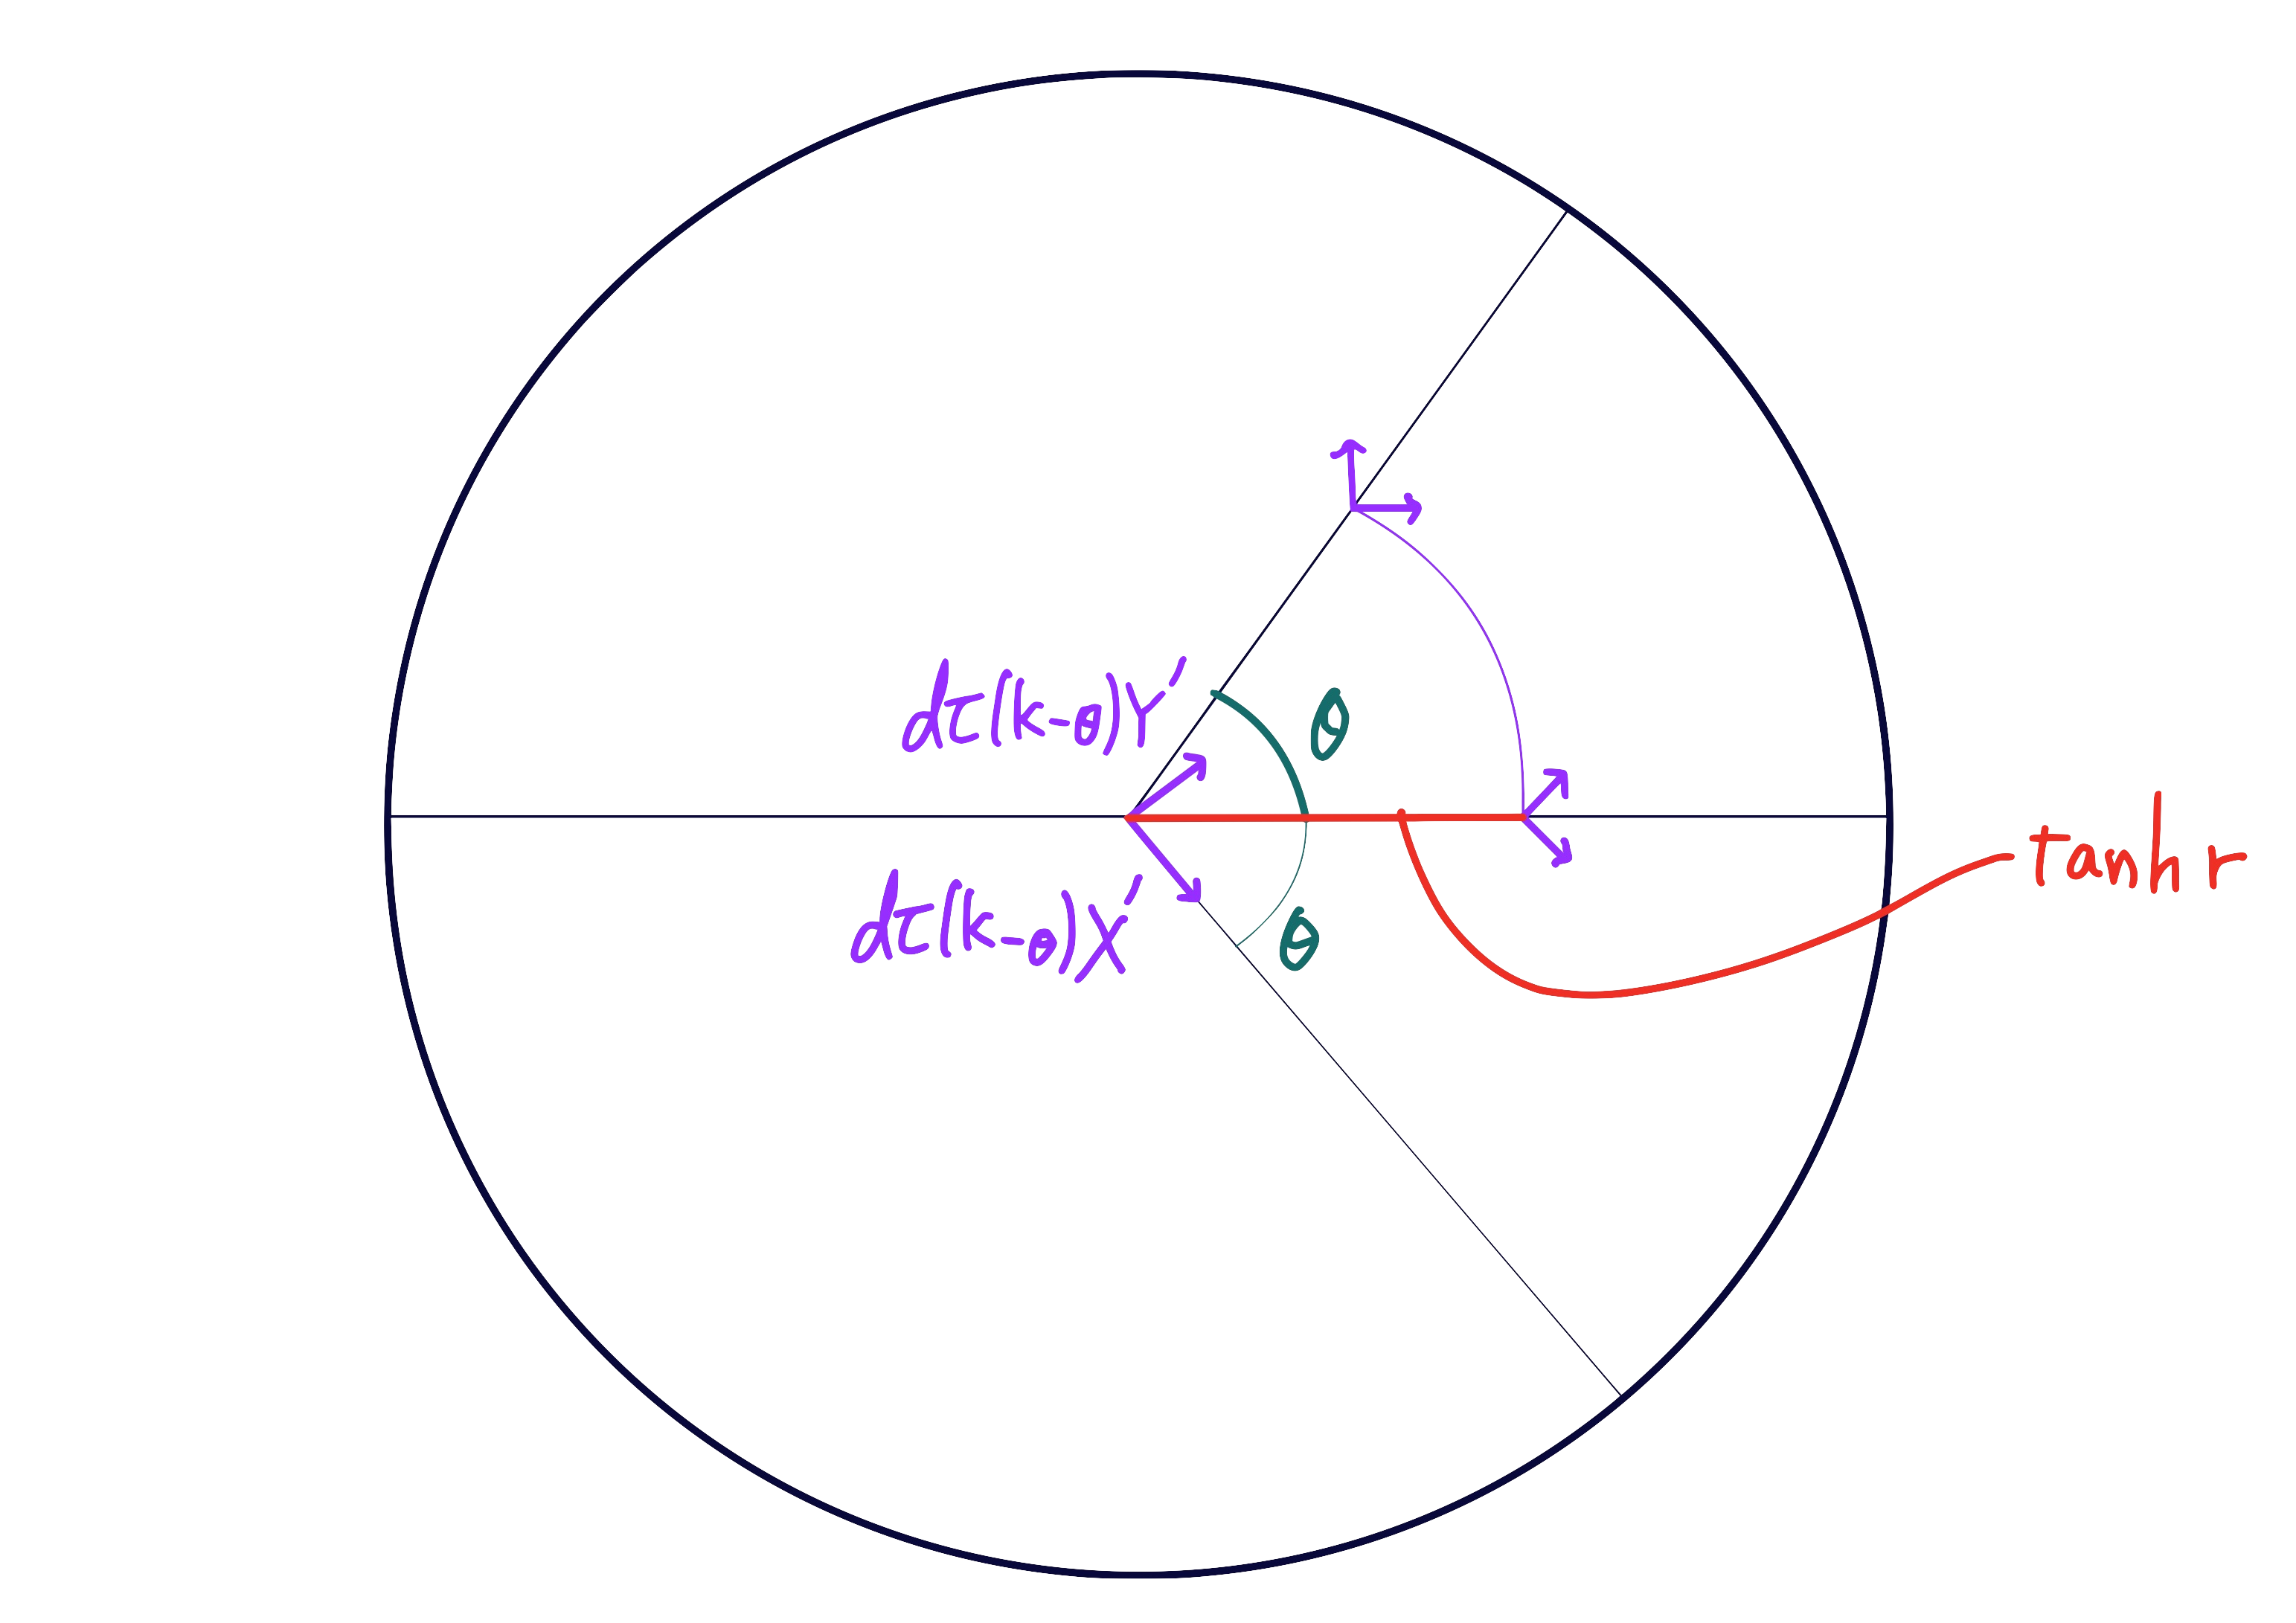
\includegraphics[scale=0.08]{../graph/riem-su11.png}
  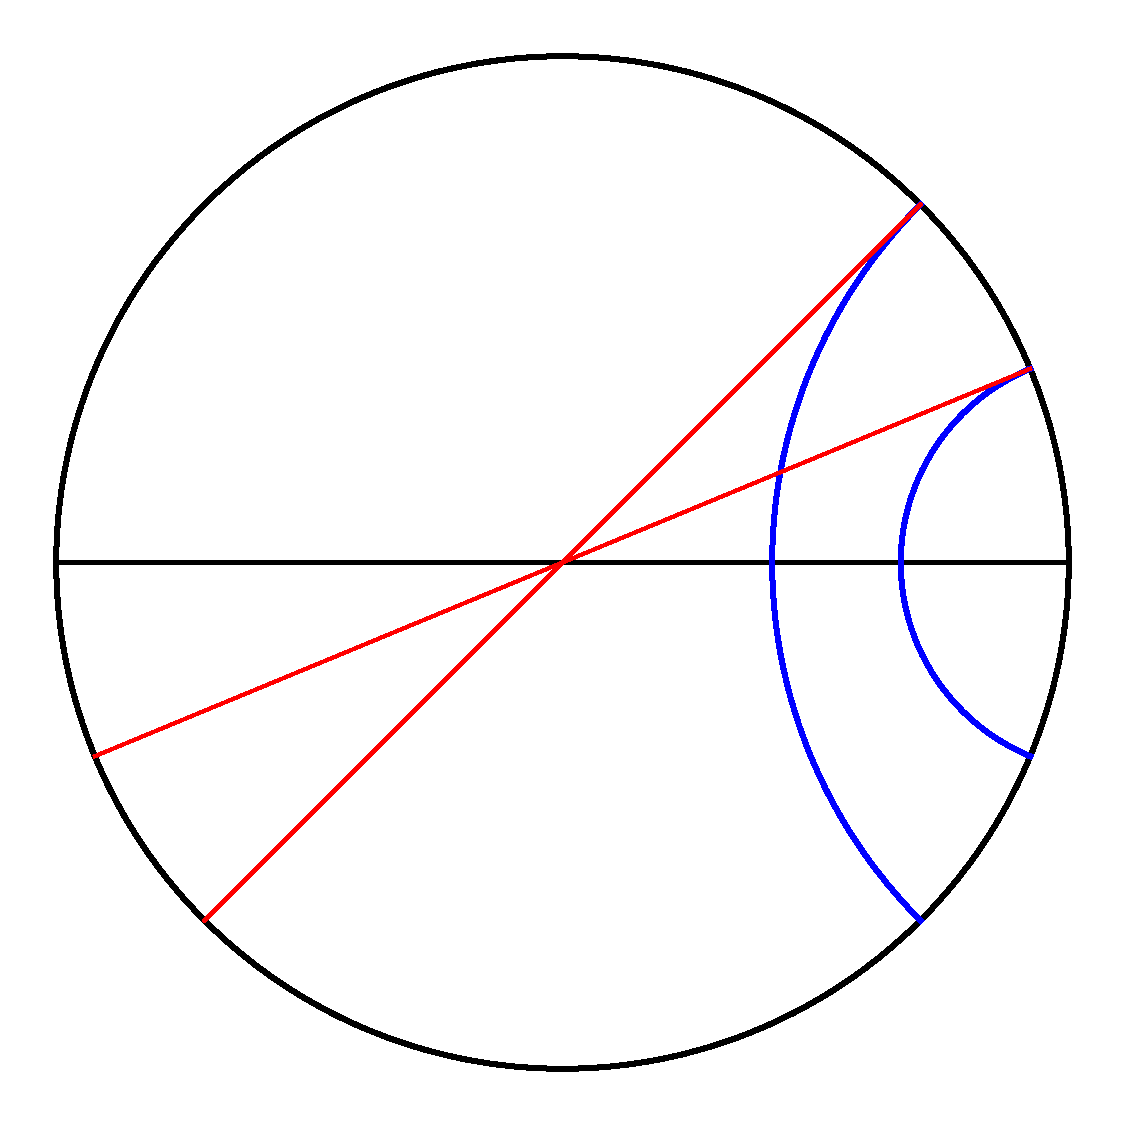
\includegraphics[scale=0.3]{../graph/visibility.pdf}
  \caption{visibility manifoldのイメージ}
  \label{fig:visibility}
\end{figure}


\begin{thm}{\cite[p.~296, 9.33~Theorem]{bh99}, originally \cite[Theorem~4.1]{e72-2}}\label{thm:visibility-and-rank}
  
  $\exists C\cptsub M\st M = \bigcup\{f(C)\mid f\in \isom(M) \}  $なるHadamard多様体$M$に対し,次は同値である.
  \vspace{-1em}
  \begin{enumerate}
    \renewcommand{\labelenumi}{(\roman{enumi})}
  \item $M$はvisibility manifoldである.
  \item 全測地的な部分Riemann多様体$M'\subset M$で$\real^2$と等長同型なものが存在しない.
  \end{enumerate}
\end{thm}

ここでRiemann対称空間はHadamard多様体であり,\Cref{thm:visibility-and-rank}の (ii) は$G$の実階数が1以下であることと同値である.したがって$G$の実階数が1の場合$G/K$はvisibility manifoldであり,$G = \SU(1,2) $,$H= \SO(1,1)$の場合の証明と全く同様にして背理法により\Cref{yosou:1121}が示される.
